\documentclass[journal]{IEEEtran}
\usepackage{graphicx}
\usepackage{url}
\title{ARGUS: Evidence Consistency Verification and Interpretable Severity Tooling for Offline CCTV Review}
\author{Munis Aparji V S, Mithin Sagar S, and Janit B\\Guide: Dr. Premanand V\\School of Computer Science and Engineering, Vellore Institute of Technology}
\begin{document}
\maketitle
\begin{abstract}
ARGUS is an implemented offline research pipeline that combines temporal detection interfaces, symbolic evidence, structured language claims, conservative verification, interpretable severity factors, and a validated recommendation vocabulary. The delivered demonstration uses eight synthetic scenes and authored language fixtures. It exercises the full operator workflow without downloaded model weights. Research adapters provide a trainable temporal transformer and a constrained ordinal severity fitter. Benchmark detection performance, human severity calibration, independent annotation agreement, and real vision-language-model ablations remain pending. The paper distinguishes executed software checks from future empirical claims.
\end{abstract}
\section{Domain and Problem Statement}
An anomaly score alone does not explain an incident. A fluent description may add objects, interactions or intent that the evidence cannot establish. ARGUS records each handoff and exposes rejected and downgraded claims. It excludes biometric identification, cross-camera re-identification, live-stream inference and automated dispatch. The automatic terminal state is awaiting human confirmation.
\section{Literature Review}
Surveillance video-language understanding supplies the conceptual task family \cite{ref1}. Prompt-enhanced weak supervision supplies a reproducible detector comparator \cite{ref2}. Graded violence assessment already exists \cite{ref3}; tracking quality is also established prior work \cite{ref4}. Normalization and snippet attention inform design choices \cite{ref5,ref6}. The broader comparison set covers graph learning, temporal constraints, feature tuning, instance models, confidence-aware prototypes, multimodal text guidance, reconstruction and open-vocabulary detection \cite{ref7,ref8,ref9,ref10,ref11,ref12,ref13,ref14,ref15}. DOI metadata has been resolved through Crossref. ARGUS does not claim these established methods as novel, reproduce every comparator, or equate metadata review with a full experimental replication.
\section{Design of Proposed Methodology}
One versioned IncidentRecord carries source provenance and seven stage outputs. M1 resamples at 25 fps and aggregates 16-frame snippets. M2 is a four-layer temporal transformer trained with binary video-level Multiple Instance Learning, LayerNorm, attention pooling and an erasing regularizer. It does not infer thirteen semantic categories from binary labels. M3 independently extracts detections and clip-local geometric tracks. M4 consumes or generates strict structured claims. M5 sees claims and evidence but not the generation prompt. Object and count checks are time-local, and unsupported action or intent assertions become inference. A narrow sentence grammar limits what can be verified.
\section{Module Description and System Design}
M6 aggregates nonnegative contributions from thirteen factors. Only independently supported observations contribute. Context and event factors without an independent verifier remain unavailable. A constrained cumulative logistic objective and score-error term fit weights from independent training ratings. Fixed ordered cut points map scores to four bands. M7 selects from twelve permitted tokens and counts invalid proposals before stripping. The operator console includes video overlays, a visible claim ledger, source-factor links, structured traces, annotation and audit screens. SQLite transactions bind decisions to append-only chained audit records. Local session names are not authenticated identities.
\section{Executed Checks}
The following values come from the sample evaluation artifact. They are synthetic software checks, not UCF-Crime or XD-Violence results and not measured human agreement.
\begin{table}[h]\centering\caption{Executed synthetic checks}\begin{tabular}{lr}
\hline
Synthetic software check & Measured value \\
\hline
Scenes & 8 \\
Authored claims & 15 \\
Rejected claims & 2 \\
Policy violations & 0 \\
Invalid actions stripped & 4 \\
\hline
\end{tabular}
\end{table}
\begin{figure}[h]\centering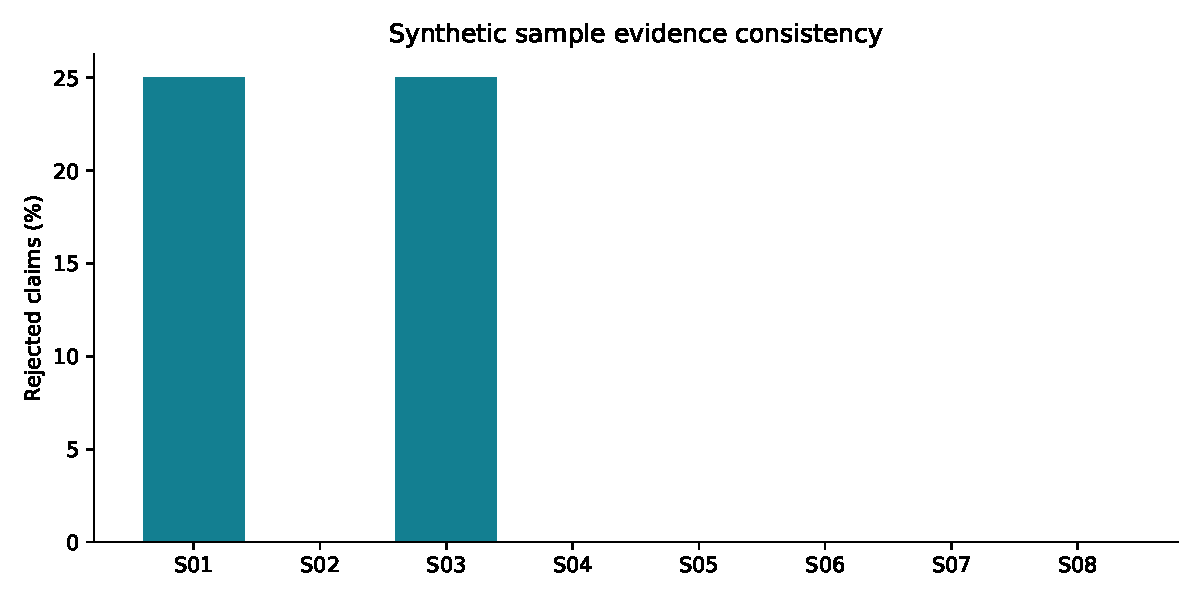
\includegraphics[width=\linewidth]{../../artifacts/figures/sample_verification.pdf}\caption{Claim rejection in authored synthetic fixtures.}\end{figure}
\section{Evaluation Plan and Limitations}
Frame-level UCF AUC requires independent test labels and correct temporal feature alignment. XD-Violence remains held out and uses AP. UCA supports temporal overlap evaluation. SIRB requires independent ratings, 20 percent overlap, pre-adjudication agreement and a source-grouped held-out split. VLM ablations compare 7B and 3B, evidence conditioning and critic use on identical clips. No target number is reported as a measured result. Detector errors can reject true claims or support false ones. The symbolic critic is not a complete semantic verifier. Unavailable factors can lower scores. Vocabulary membership does not establish response appropriateness. The package is local academic software, not a validated security product.
\bibliographystyle{IEEEtran}
\bibliography{references}
\end{document}
